\documentclass[11pt, aspectratio=169]{beamer}
\usefonttheme[onlymath]{serif}

\setbeamersize{text margin left=1.5em}
\setbeamersize{text margin right=1.5em}

\setbeamertemplate{frametitle}{%
  \vskip1ex
  \usebeamerfont{frametitle}%
  \insertframetitle\par
  \vskip1ex
  \hrule
}

\setbeamertemplate{blocks}[rounded][shadow=true]

% Add numbered captions for figures/tables in beamer
\setbeamertemplate{caption}[numbered]

\setbeamertemplate{itemize item}{\usebeamerfont{itemize item}\textbullet}
\setbeamertemplate{itemize subitem}{\usebeamerfont{itemize subitem}\textbullet}
\setbeamertemplate{itemize subsubitem}{\usebeamerfont{itemize subsubitem}\textbullet}

\makeatletter
\geometry{%
  papersize={\fpeval{\beamer@paperwidth*1.5}pt,\fpeval{\beamer@paperheight*1.5}pt},
  hmargin=\fpeval{0.5 * 1.0}cm,% 1cm
  vmargin=0cm,%
  head=\fpeval{0.5*1.5}cm,% 0.5cm
  headsep=0pt,%
  foot=\fpeval{0.5*1.5}cm% 0.5cm
}
\makeatother

\usepackage{booktabs}
\usepackage{graphicx}
\usepackage[dvipsnames]{xcolor} % <-- removed obsolete `usenames` option
\usepackage{amsmath}
\usepackage{amssymb}
\usepackage{mathtools}
\usepackage{subcaption}

\usepackage[
  backend=bibtex,
  style=authoryear,   % or numeric
  citestyle=authoryear
]{biblatex}
\addbibresource{../../references.bib}

% Your custom commands (kept as is)
\newcommand{\mrm}[1]{\mathrm{#1}}
\newcommand{\mbb}[1]{\mathbb{#1}}
\newcommand{\mb}[1]{\mathbf{#1}}
\newcommand{\mc}[1]{\mathcal{#1}}
\newcommand{\tb}[1]{\textbf{#1}}
\newcommand{\Unif}{\operatorname{Unif}}

\DeclareMathOperator{\diverg}{div}

% \DeclareMathOperator{\div}{\operatorname{div}}

\title{Flow Matching and its usage in Offline RL}
\author{Gwanwoo Choi}
\institute{MLIC}
\date{} % To use the current date

\begin{document}

\begin{frame}
    \titlepage
\end{frame}

\begin{frame}{Flow Matching Concept}
  \begin{block}{Problem Definition}
    \begin{columns}[t]
      \begin{column}{0.45\textwidth}
        \begin{figure}
      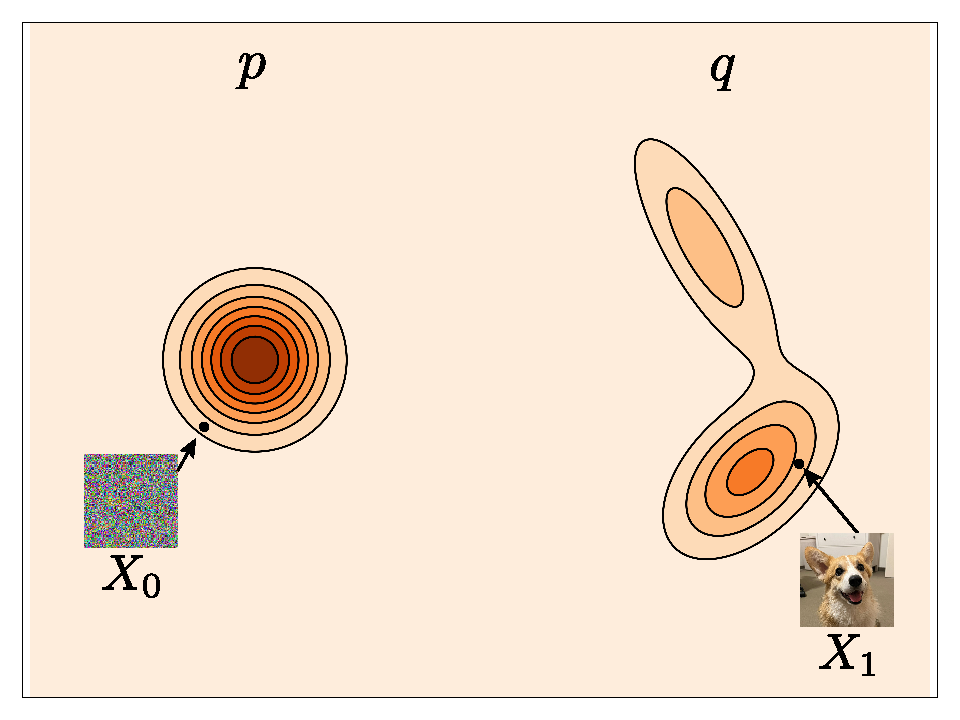
\includegraphics[width=0.6\textwidth]{assets/data.pdf}
      \caption{Data Distribution}
      \end{figure}

      \end{column}
      \begin{column}{0.50\textwidth}
        \begin{itemize}
          \item Let $q$ be the data distribution.
          \item Our objective is to \tb{learn a generative model} that can sample from $q$.
          \item Each data point is modeled as a random variable (r.v.) $X_1 \in \mathbb{R}^d$ with distribution $X_1 \sim q$.
          \item Modern generative models (e.g. VAE, Diffusion Models, Flow Matching) leverages an tractable distribution (e.g. Gaussian) to generate $X_1$.
          \item Let $q$ denote a known distribution chosen for modeling (e.g., a Gaussian), and let $X_0$ be a random variable with distribution $X_0 \sim p$.
        \end{itemize}
      \end{column}
    \end{columns}
  \end{block}
\end{frame}


\begin{frame}{Flow Matching Concept}

  \begin{block}{Differences between generative models}
    \begin{figure}
    \centering
    % Reduce spacing between the two images by using wider subfigures
    % and a small fixed horizontal gap. Keep images slightly inset with
    % includegraphics width < \subfigure width to avoid touching edges.
    \captionsetup[subfigure]{skip=0.5ex, labelfont=small, textfont=small}
    \begin{subfigure}[b]{0.30\textwidth}
      \centering
      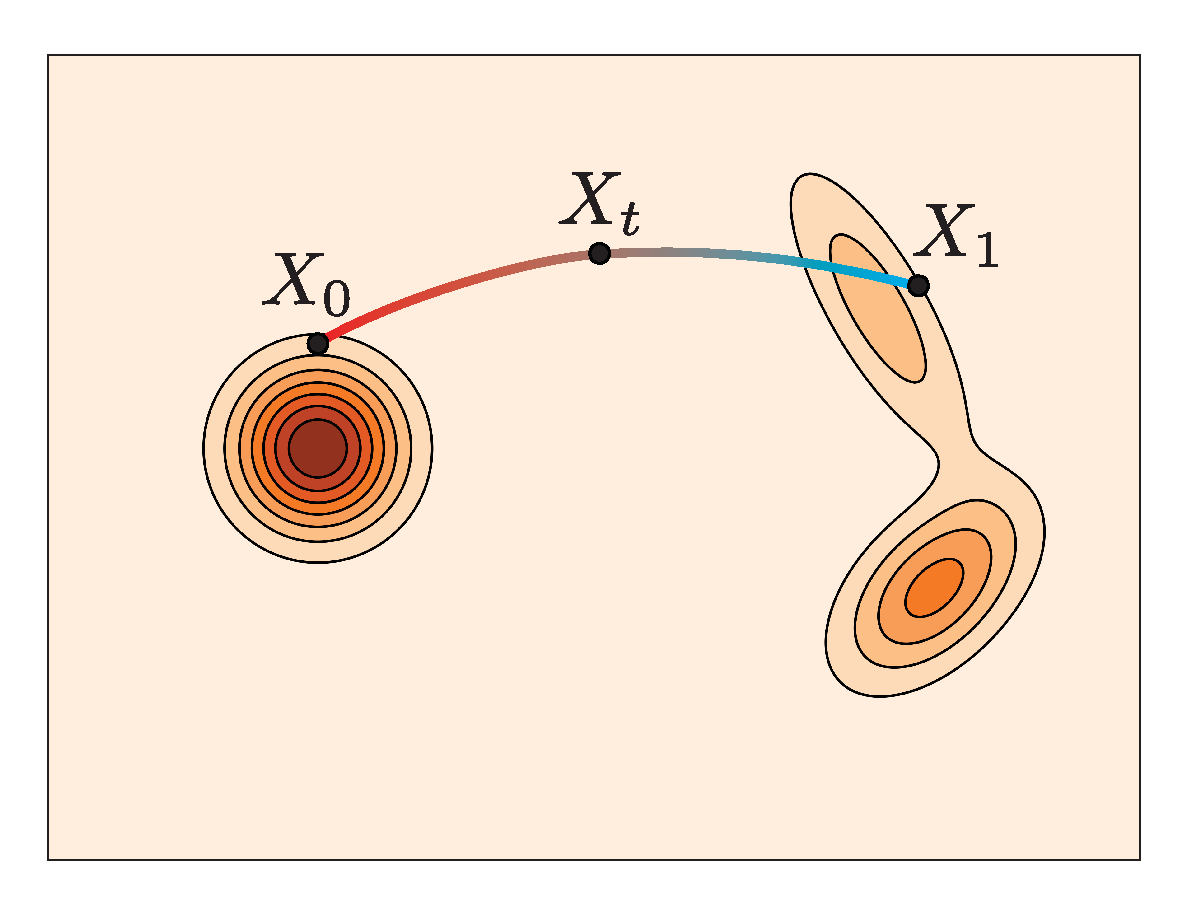
\includegraphics[width=0.9\textwidth]{assets/type_flow.pdf}
      \caption{Flow}
      \label{fig:types:flow}
    \end{subfigure}\hspace{0.02\textwidth}%
    \begin{subfigure}[b]{0.30\textwidth}
      \centering
      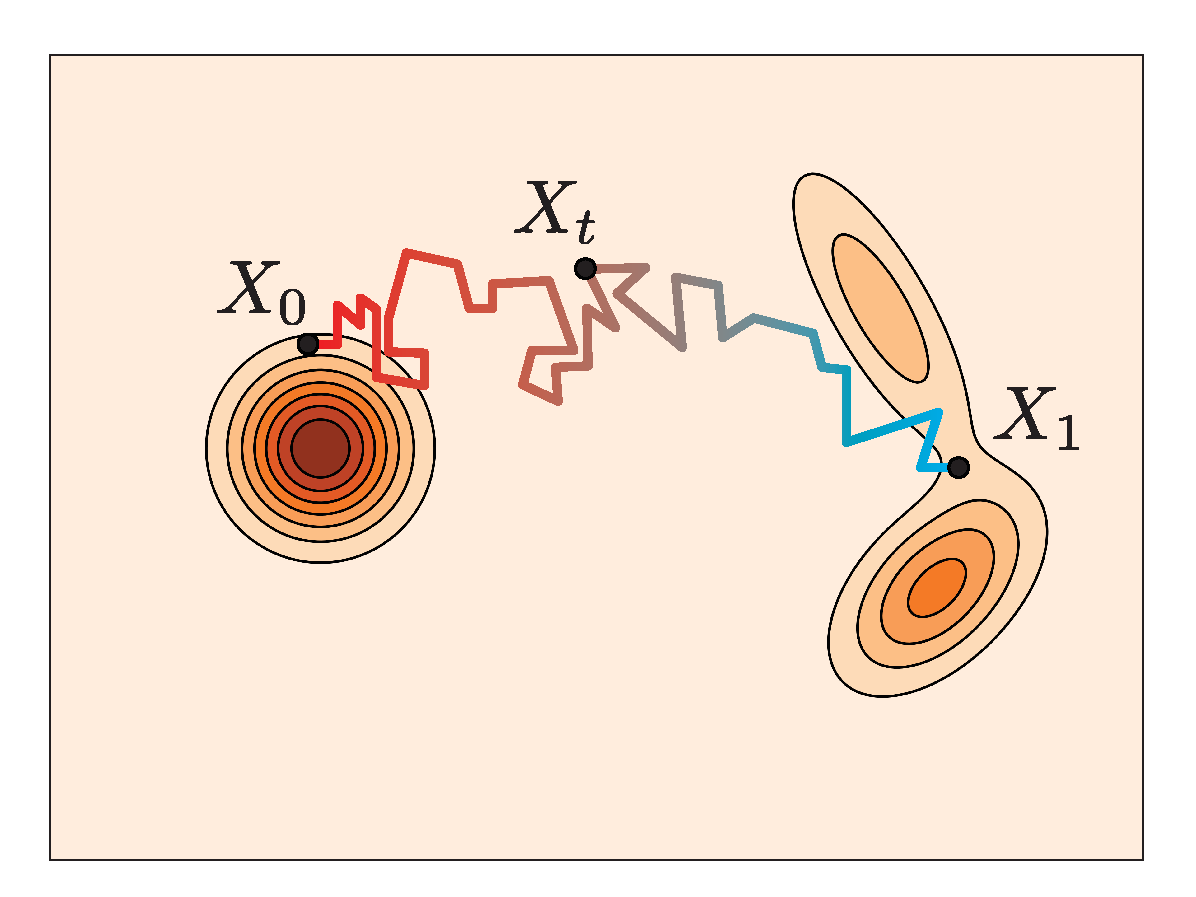
\includegraphics[width=0.9\textwidth]{assets/type_diffusion.pdf}
      \caption{Diffusion}
      \label{fig:types:diffusion}
    \end{subfigure}
    \caption{Difference between Flow Matching and Diffusion Models}
    \end{figure}

    \begin{itemize}
      \item Variational AutoEncoders (VAE): sample $x_0$ from a prior and use a deterministic decoder to produce $X_1$.
      \item Flow Matching: Construct a deterministic continuous flow (ODE-based) that transports $X_0$ to $X_1$.
      \item Diffusion models: generate $X_1$ by simulating a stochastic process (e.g. reverse-time SDE), so the mapping from $X_0$ to $X_1$ is stochastic.
    \end{itemize}
  \end{block}
\end{frame}

\begin{frame}{Flow Matching Concept}
  \begin{block}{Probability Path}
    \begin{columns}
      \begin{column}{0.45\textwidth}
        \begin{figure}
          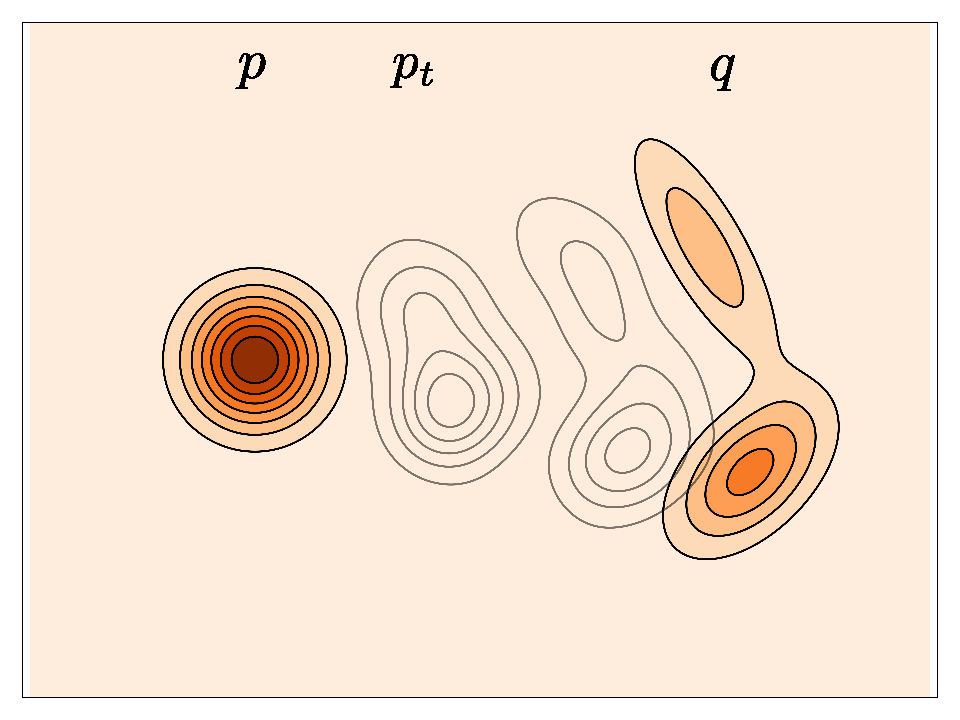
\includegraphics[width=0.6\textwidth]{assets/p_t.pdf}
        \end{figure}
      \end{column}
      \begin{column}{0.50\textwidth}
        \begin{itemize}
          \item Let define a \tb{probability path} $(p_t)_{0 \leq t \leq 1}$.
          \item The path $p_t$ is a \underline{continuous interpolation} between the known distribution $p$ and the data distribution $q$ such that $p_{0} = p$ and $p_{1} = q$.
          \item How can we find \underline{proper} $p_t$ for all $t \in [0,1]$ that matches boundary condition $p_0= p, p_1 = q$? ($\to$ Flow Matching.)
        \end{itemize}
      \end{column}
    \end{columns}
  \end{block}
\end{frame}

\begin{frame}{Basic Concept}
  \begin{block}{Flow \& Flow Model}
    \begin{itemize}
      \item A $C^r$ \tb{flow} is a \underline{time-dependent positional mapping} $\psi: [0,1] \times \mbb{R}^d \to \mbb{R}^d$ (here $C^r$ denotes functions whose derivatives up to order $r$ exist and are continuous).
      \item Let denote $\psi_t(x)$ as the \underline{position at time $t$ of a particle} that started at $x$ at time $t=0$ ($\psi: (t,x) \mapsto \psi_t(x)$).
      \item $\psi \in C^r$ and $\psi_t$ is a $C^r$ diffeomorphism.
      \item A \tb{Flow Model} is a \hyperlink{appendix:flow_model_markov}{\underline{continuous-time Markov process}} $(X_t)_{0 \leq t \leq 1}$ defined by applying a flow $\psi_t$ to the RV $X_0$.
      $$
        X_t = \psi_t(X_0),\ t \in [0,1], \text{ where } X_0 \sim p
      $$
      \item The \tb{goal of generative flow modeling} is to find a flow $\psi_t$ such that 
      $$
        X_1 = \psi_1 (X_0) \sim q
      $$
    \end{itemize}
  \end{block}

  \begin{block}{Samples of Flow Model}
    \begin{figure}
      \centering
      \captionsetup[subfigure]{skip=0.5ex, labelfont=small, textfont=small}
      \begin{subfigure}[b]{0.23\textwidth}
        \centering
        \includegraphics[width=0.9\textwidth]{assets/flow_1_p.png}
        \caption{$X_0$}
      \end{subfigure}\hspace{0.02\textwidth}
      \begin{subfigure}[b]{0.23\textwidth}
        \centering
        \includegraphics[width=0.9\textwidth]{assets/flow_10_p.png}
        \caption{$X_t = \psi_t(X_0)$}
      \end{subfigure}\hspace{0.02\textwidth}
      \begin{subfigure}[b]{0.23\textwidth}
        \centering
        \includegraphics[width=0.9\textwidth]{assets/flow_16_p.png}
        \caption{$X_1 = \psi_1(X_0)$}
      \end{subfigure}
    \end{figure}
  \end{block}
\end{frame}

\begin{frame}{Basic Concept}
  \begin{block}{Equivalence between flows and velocity fields}
    \begin{itemize}
      \item Let denote $u_t(x)$ as the \underline{velocity} of a particle, which is positioned in $x$ at time $t=0$, at time $t$.
      \item A flow $\psi$ be defined in terms of a \tb{velocity field} $u: [0,1] \times \mbb{R}^d \to \mbb{R}^d$ via the following ODE:
      $$
      \begin{gathered}
        \frac{d}{dt} \psi_t(x) = u_t(\psi_t(x)) \\
        \psi_0(x) = x
      \end{gathered}
      $$
    \end{itemize}
  \end{block}

  \begin{block}{Velocity fields}
    \begin{figure}
      \centering
      \captionsetup[subfigure]{skip=0.5ex, labelfont=small, textfont=small}
      \begin{subfigure}[b]{0.23\textwidth}
        \centering
        \includegraphics[width=0.9\textwidth]{assets/flow_1.png}
        \caption{$u_0$}
      \end{subfigure}\hspace{0.02\textwidth}
      \begin{subfigure}[b]{0.23\textwidth}
        \centering
        \includegraphics[width=0.9\textwidth]{assets/flow_10.png}
        \caption{$u_t$}
      \end{subfigure}\hspace{0.02\textwidth}
      \begin{subfigure}[b]{0.23\textwidth}
        \centering
        \includegraphics[width=0.9\textwidth]{assets/flow_16.png}
        \caption{$u_1$}
      \end{subfigure}
    \end{figure}
  \end{block}
\end{frame}

\begin{frame}{Basic Concept}
  \begin{block}{Push-forward (Change of variables)}
    \begin{itemize}
      \item \tb{Push-forward} describes how a probability \underline{distribution transforms under a mapping}.
      \item Given a RV $X \sim p_X$ with density $p_X$, let us consider a RV $Y = f(X)$, where $f: \mbb{R}^d \to \mbb{R}^d$ is a $C^1$ diffeomorphism and let $g = f^{-1}$ be its inverse mapping.
      \item The probability density function(PDF) of $Y$ is called the \tb{push-forward} of $p_X$ and denoted by $$[f_{\#}p_X](y) \triangleq p_X(f^{-1}(y))\lvert \det \partial_y \phi(y)\rvert= p_Y(y), \quad  \text{ where }[\partial_y g(y)]_{i,j} = \frac{\partial g^i}{\partial y^j}, i,j \in \{1,2,\dots, d\}$$
    \end{itemize}
  \end{block}

  \begin{block}{Probability Paths}
    \begin{columns}
      \begin{column}{0.3\textwidth}
        \begin{figure}
          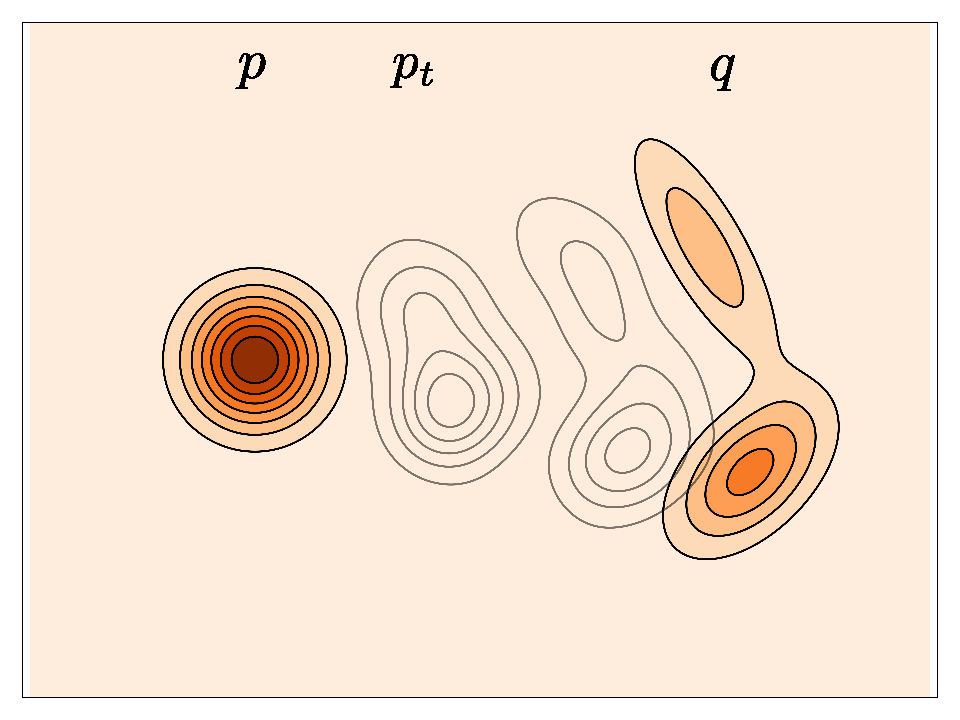
\includegraphics[width=0.9\textwidth]{assets/p_t.pdf}
        \end{figure}
      \end{column}
      \begin{column}{0.65\textwidth}
        \begin{itemize}
          \item We call a time-dependent probability $(p_t)_{0 \leq t \leq 1}$ a \tb{probability path}.
          \item For each time $t\in [0,1]$, these marginal PDFs are obtained via the push-forward formula
          $$
            p_t(x) = [\psi_{t \#} p](x)
          $$
          \item We call that $u_t$ \tb{generates} $p_t$ if $X_t = \psi_t(X_0) \sim p_t$ for all $t \in [0,1)$.
          \item The condition that $u_t$ can be generate $p_t$ is described in \hyperlink{appendix:continuity_equation_and_mass_conservation}{Appendix}.
        \end{itemize}
      \end{column}
    \end{columns}
  \end{block}
\end{frame}

\begin{frame}{Flow Matching}
  \begin{block}{Flow Matching Problem}
    \begin{itemize}
      \item Given a source distribution $p$ and a target distribution $q$, Flow Matching (FM) is a scalable approach for training a flow model, defined by a learnable velocity $u^\theta_t$. and solving the \tb{Folw Matching Problem}
    \end{itemize}
  \end{block}
\end{frame}


\begin{frame}{Appendix}

  \begin{block}{$C^r$ diffeomorphism} \label{appendix:diffeomorphism}
    We denote by $C^r(\mbb{R}^m, \mbb{R}^n)$ the collection of functions $f: \mbb{R}^m \to \mbb{R}^n$ with continuous derivatives of order $r$:
    $$
      \frac{\partial^r f^k}{\partial x^{i_1} \cdots \partial x^{i_r}}, \quad k \in \{1,2,\dots, n\}, i_j \in \{1, 2, \dots, m\}
    $$
    A map $f: \mbb{R}^n \to \mbb{R}^n$ is a $C^r$ \tb{diffeomorphism} if $f \in C^r(\mbb{R}^n, \mbb{R}^n)$ and its inverse $f^{-1}$ exists and satisfies $f^{-1} \in C^r(\mbb{R}^n, \mbb{R}^n)$.
  \end{block}
  \begin{block}{Flow Model is a Markov process} \label{appendix:flow_model_markov}
    $$
      X_s = \psi_s(X_0) = \psi_s (\psi^{-1}(\psi_t(X_0))) = \psi_{s|t}(X_t), \text{ where } \psi_{s|t} \triangleq \psi_s \circ \psi_t^{-1}
    $$
  \end{block}
\end{frame}

\begin{frame}{Appendix}
    \begin{block}{Continuity Equation and Mass Conservation} \label{appendix:continuity_equation_and_mass_conservation}
    To verify that a velocity field $u_t$ generates a probability path $p_t$, one can verify if the pair $(u_t, p_t)$ satisfies a partial differential equation (PDE) known as the \underline{Continuity Equation}:
    $$
      \frac{d}{dt}p_t(x) + \diverg(p_t u_t)(x) = 0
    $$
    where $\diverg(v)(x) = \sum^d_{i=1} \partial_{x^i} v^i(x)$, and $v(x) = (v^1(x), \dots, v^d(x))$.

    The following theorem, a rephrased version of the \underline{Math Conservation Formula}, states that a solution $u_t$ to the Continuity Equation generates the probability path $p_t$

    \begin{theorem}[Mass Conservation]
      Let $p_t$ be a probability path and $u_t$ a locally Lipchitz integrable vector field. Then, the following two statements are equivalent:
      \begin{enumerate}
        \item The Continuity Equation holds for $t \in [0,1)$
        \item $u_t$ generates $p_t$
      \end{enumerate}
    \end{theorem}
  \end{block}
\end{frame}

\end{document}